\documentclass[12pt, a4paper]{article}

% --- Pacotes ---
\usepackage[utf8]{inputenc}
\usepackage[T1]{fontenc}
\usepackage[brazilian]{babel}
\usepackage{graphicx}
\usepackage{float}
\usepackage{booktabs}
\usepackage{amsmath}
\usepackage{hyperref}
\usepackage[margin=2.5cm]{geometry}
\usepackage{caption}
\usepackage{subcaption}
\usepackage{array}
\usepackage{xcolor}

% --- Caminho das imagens ---
\graphicspath{{imagens/}}

% --- Dados do documento ---
\title{\textbf{Lab. 2 -- Criação de Classificadores baseado em Dados} \\[0.5cm]
\large CMC-13 -- Introdução a Ciência de Dados}
\author{
  Lucas Saorin \\
  João Victor Saraiva Rodrigues \\
  Fabio Eiiti Kobayashi Urio
}
\date{\today}

% =============================================================================
\begin{document}
\maketitle
\tableofcontents
\newpage

% =============================================================================
\section{Preparação dos Dados}

\subsection{Descrição do Dataset}

O conjunto de dados tem como objetivo prever a rotatividade de clientes (\textit{customer churn}).
A variável alvo é \texttt{Churn} (0 = cancelou o serviço, 1 = não cancelou).
Os dados foram fornecidos em dois arquivos separados:

\begin{itemize}
  \item \textbf{Treino:} 440.832 amostras × 12 colunas
  \item \textbf{Teste:}  64.374 amostras × 12 colunas
\end{itemize}

As features originais são: \texttt{CustomerID}, \texttt{Age}, \texttt{Gender},
\texttt{Tenure}, \texttt{Usage Frequency}, \texttt{Support Calls},
\texttt{Payment Delay}, \texttt{Subscription Type}, \texttt{Contract Length},
\texttt{Total Spend} e \texttt{Last Interaction}.

A taxa de churn no treino é de 56,7\% e no teste de 47,4\%, indicando uma diferença
de distribuição entre os conjuntos que, como será discutido adiante, influenciou
diretamente o desempenho dos modelos.

% -----------------------------------------------------------------------------
\subsection{Limpeza Inicial}

Foram aplicadas as seguintes transformações antes da análise exploratória:

\begin{enumerate}
  \item \textbf{Remoção de linhas vazias:} encontrada 1 linha completamente vazia
        no conjunto de treino (índice 199.295), removida via \texttt{dropna(how='all')}.

  \item \textbf{Remoção de \texttt{CustomerID}:} identificador único sem valor preditivo.

  \item \textbf{Conversão \texttt{float} → \texttt{int} no treino:} artefato da linha
        NaN removida. Após a remoção, colunas que deveriam ser inteiras passaram a
        ter dtype \texttt{float64}. A conversão explícita restaurou o tipo correto e
        alinhou a granularidade com o conjunto de teste.
\end{enumerate}

% -----------------------------------------------------------------------------
\subsection{Codificação de Variáveis Categóricas}

Três variáveis categóricas foram codificadas antes da exportação dos dados:

\begin{itemize}
  \item \textbf{\texttt{Gender}:} codificação binária (Male = 0, Female = 1).

  \item \textbf{\texttt{Contract Length}:} codificação ordinal respeitando a ordem
        natural de duração (Monthly = 1, Quarterly = 3, Annual = 12).

  \item \textbf{\texttt{Subscription Type}:} \textit{one-hot encoding} com
        \texttt{drop\_first=True}, gerando as colunas \texttt{Subscription Type\_Premium}
        e \texttt{Subscription Type\_Standard}. A categoria \textit{Basic} torna-se a
        referência implícita.
\end{itemize}

% -----------------------------------------------------------------------------
\subsection{Análise Exploratória}

A análise exploratória abrangeu histogramas, curvas KDE e boxplots para as sete
features contínuas (\texttt{Age}, \texttt{Tenure}, \texttt{Usage Frequency},
\texttt{Support Calls}, \texttt{Payment Delay}, \texttt{Total Spend},
\texttt{Last Interaction}), sempre com treino e teste lado a lado para detectar
eventuais diferenças de distribuição.

A Figura~\ref{fig:dist_churn} exibe a distribuição de cada feature segmentada
por classe de churn. Observa-se que \texttt{Support Calls} e \texttt{Total Spend}
apresentam a separação mais nítida entre as classes: clientes que cancelaram tendem
a ter mais chamadas de suporte e menor gasto total. \texttt{Payment Delay} e
\texttt{Age} mostram separação moderada; as demais features apresentam distribuições
muito sobrepostas.

\begin{figure}[H]
  \centering
  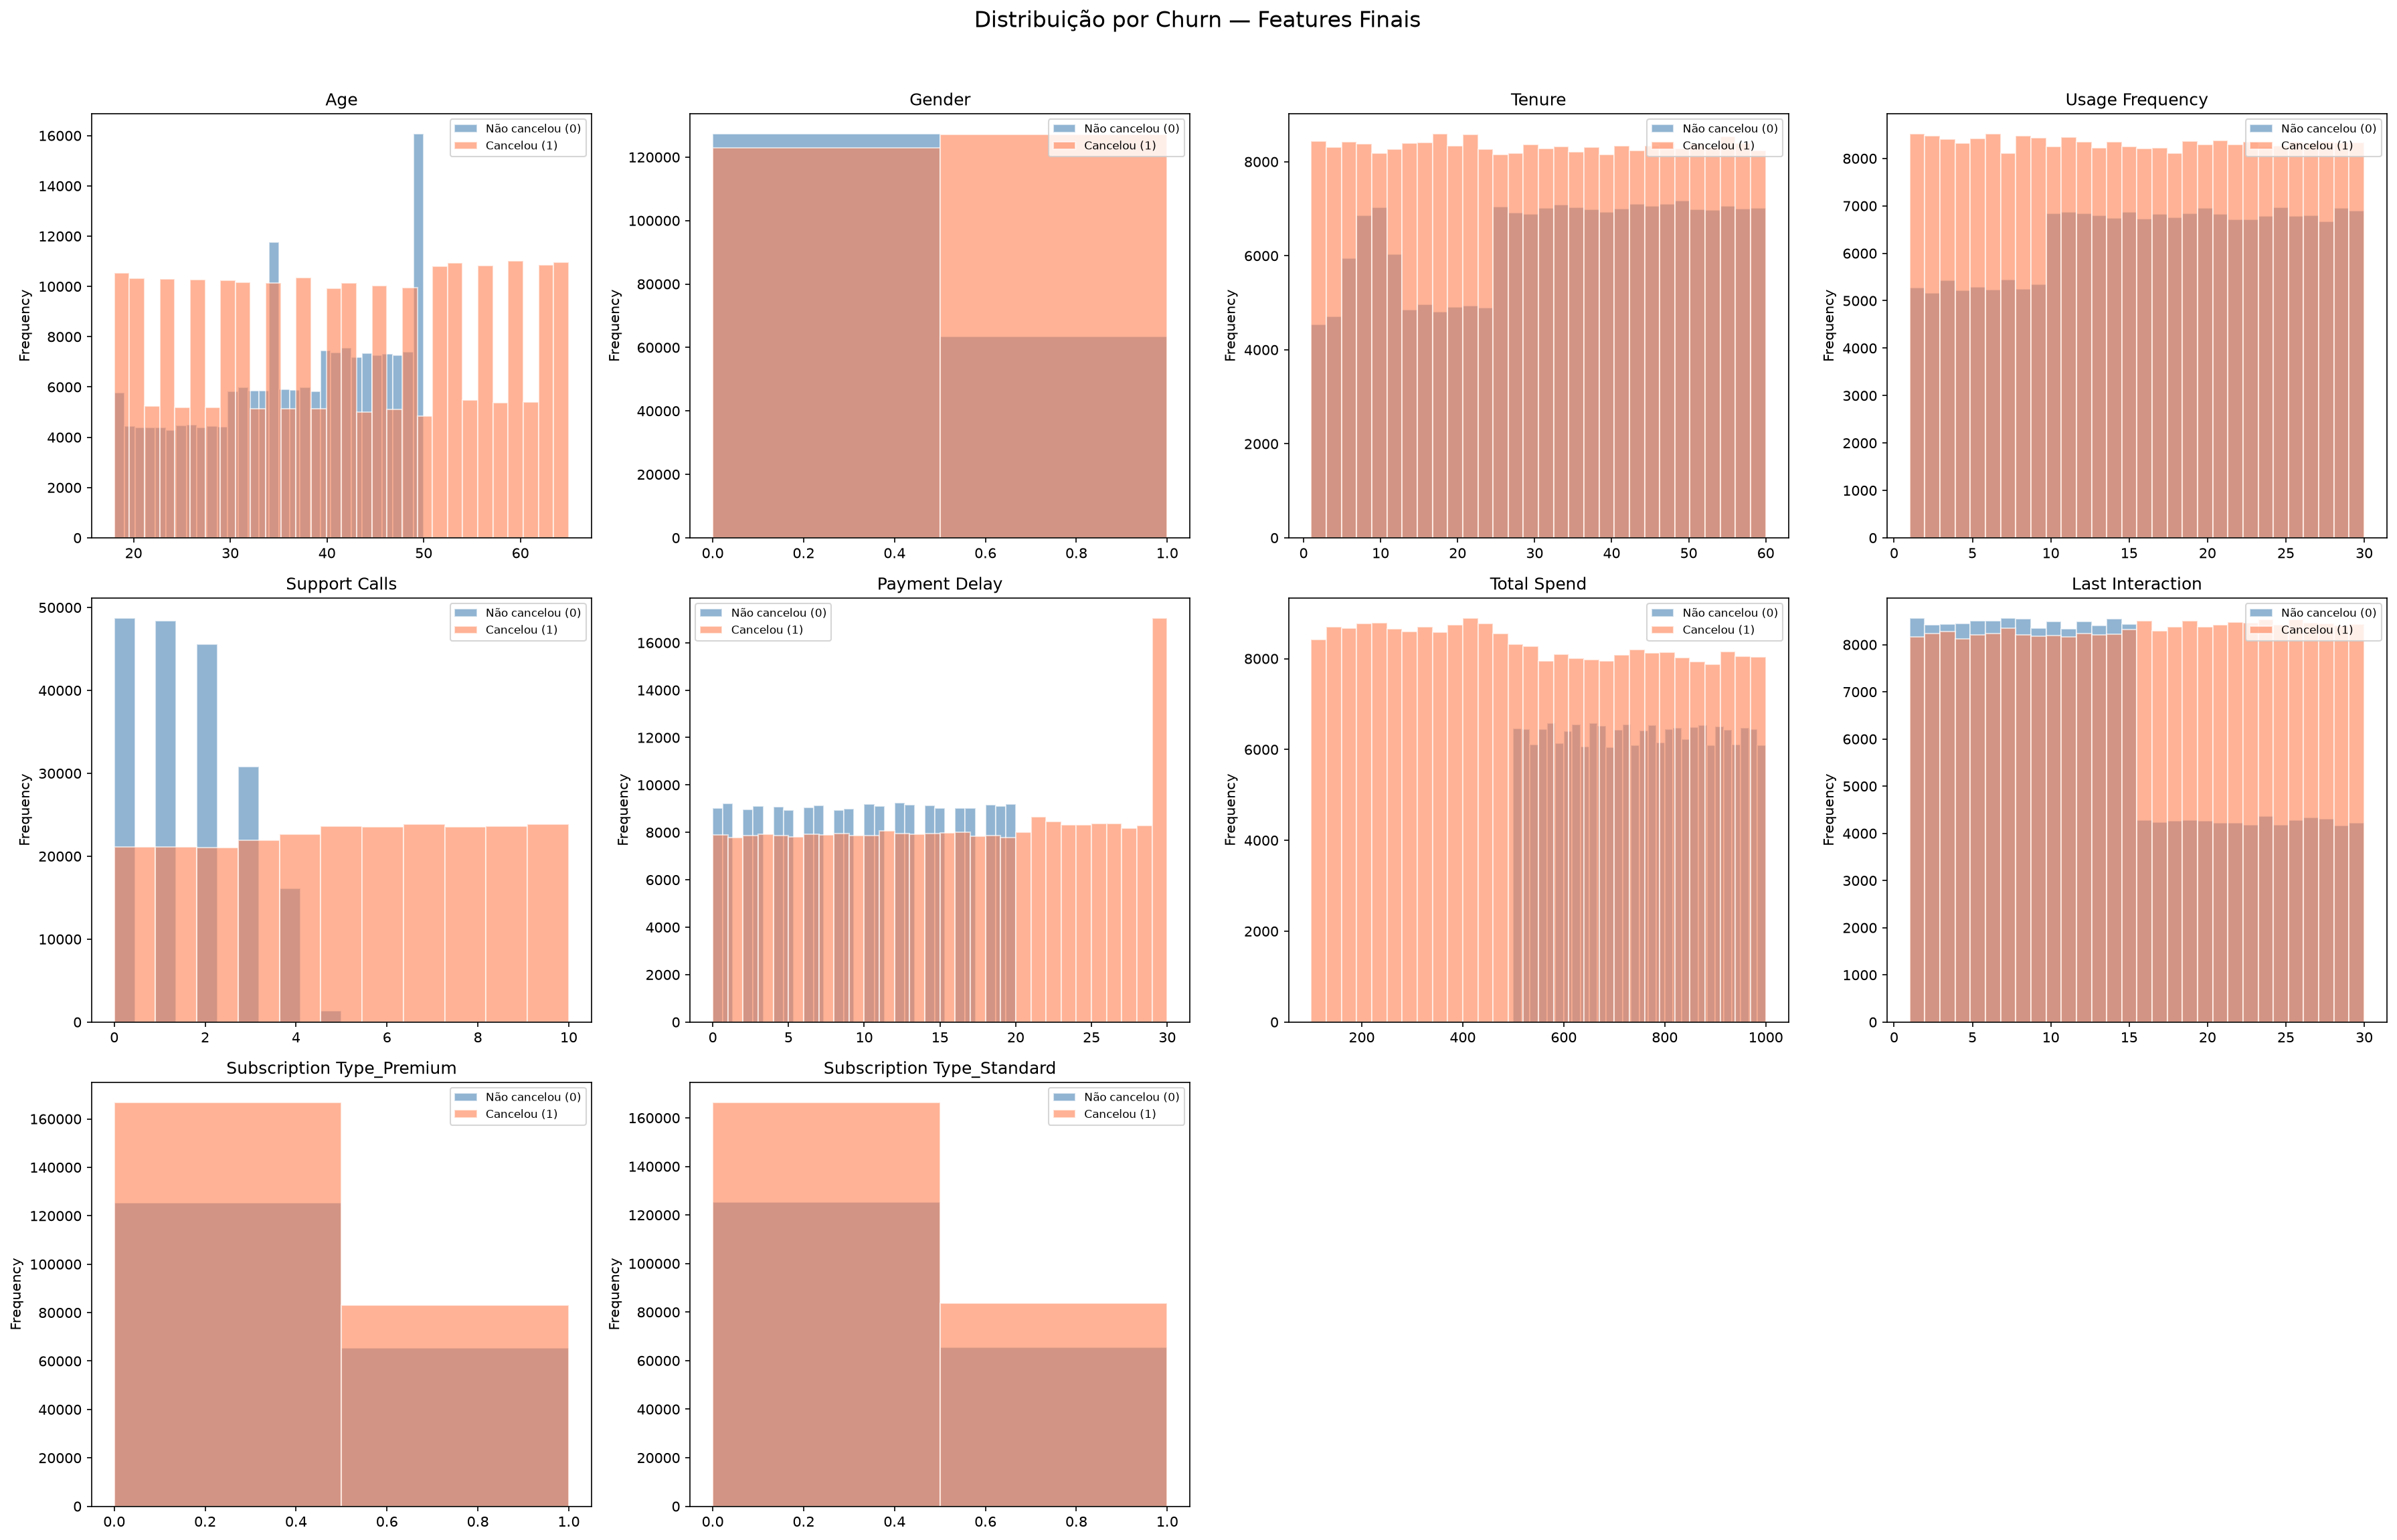
\includegraphics[width=\textwidth]{1_prep_churn_features_finais.png}
  \caption{Distribuição das features por classe de churn (Churn=0 vs Churn=1) no conjunto de treino.}
  \label{fig:dist_churn}
\end{figure}

% -----------------------------------------------------------------------------
\subsection{Investigação de Problemas}

\subsubsection{Separação Perfeita em \texttt{Contract Length}}

Durante a análise de distribuição por churn, identificou-se um comportamento crítico
em \texttt{Contract Length}: contratos \textit{Monthly} apresentam taxa de churn de
\textbf{100\%} no conjunto de treino (87.104 amostras), porém apenas \textbf{51,6\%}
no conjunto de teste (22.130 amostras). Quarterly e Annual mantêm comportamento
consistente entre treino e teste ($\approx$46\%).

Essa discrepância caracteriza um \textit{distribution shift} severo: qualquer modelo
aprende a regra ``Monthly = churn garantido'' e erra metade das predições no teste
para contratos mensais. A Figura~\ref{fig:contract_shift} ilustra essa diferença.

\begin{figure}[H]
  \centering
  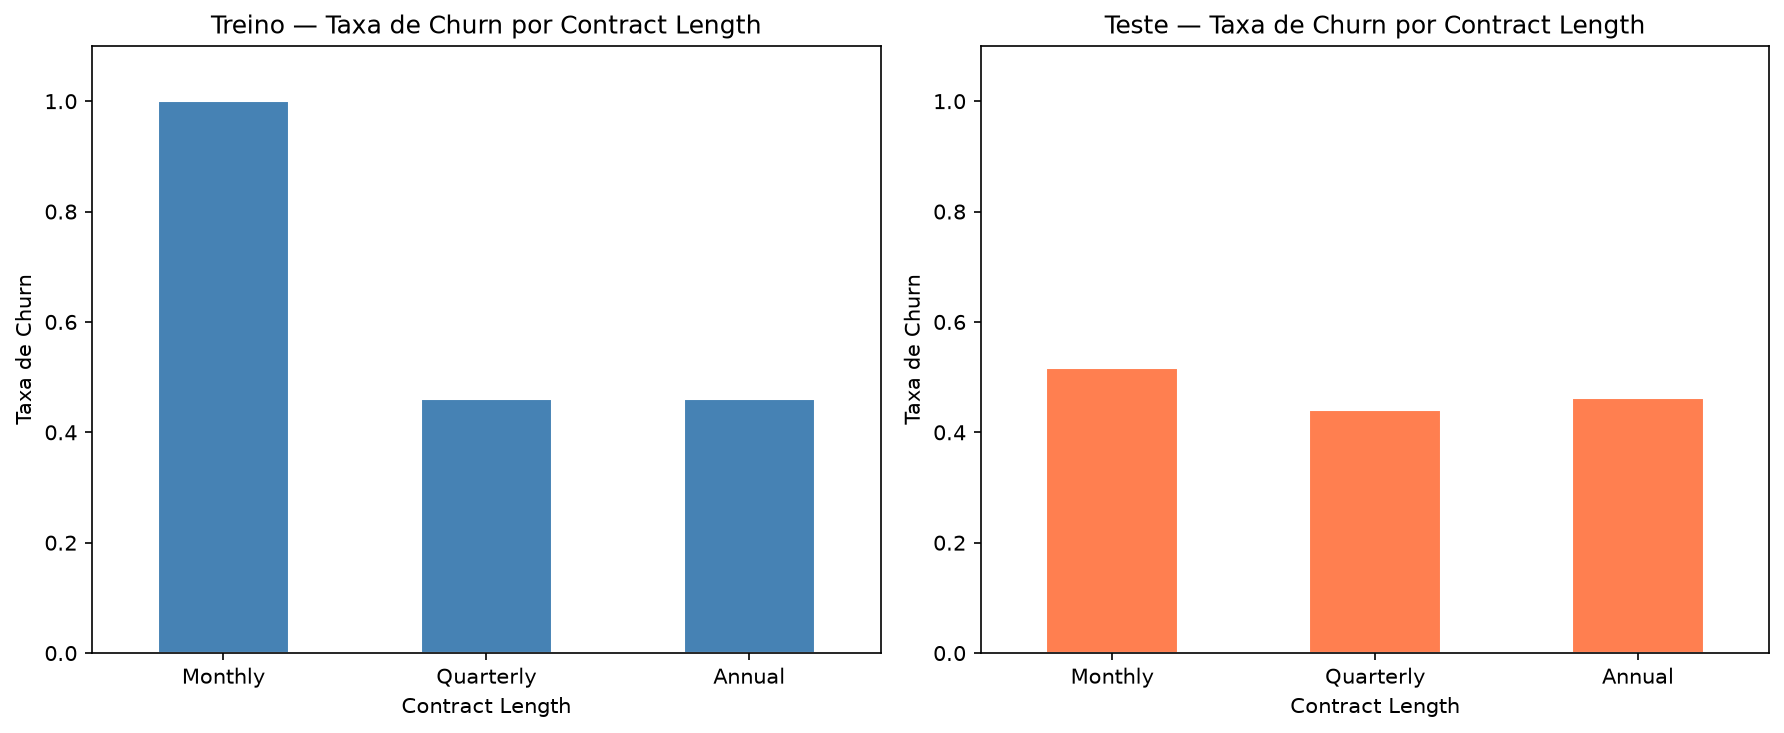
\includegraphics[width=0.85\textwidth]{1_prep_separacao_perfeita_contract.png}
  \caption{Taxa de churn por tipo de contrato no treino (esquerda) e no teste (direita).
           O comportamento de \textit{Monthly} diverge completamente entre os conjuntos.}
  \label{fig:contract_shift}
\end{figure}

Um teste adicional confirmou o impacto: uma árvore de decisão com profundidade 3
utilizando apenas \texttt{Support Calls} e \texttt{Contract Length} atingiu 84,3\%
de acurácia no treino, mas somente 61,7\% no teste (queda de 23 pp). Com todas as
features, o treino sobe para 92,2\% e o teste cai para 58,5\% --- adicionar mais
features piorou a generalização, evidenciando memorização do treino.

\textbf{Decisão:} \texttt{Contract Length} foi removida antes da exportação dos dados.
Essa foi a melhoria de maior impacto no projeto.

\subsubsection{Granularidade de \texttt{Total Spend}}

O conjunto de treino original apresentava \texttt{Total Spend} em formato \texttt{float64}
(valores como 932.0, 185.3), enquanto o teste já estava em inteiros. A conversão
\texttt{float} → \texttt{int} unificou a granularidade: ambos os conjuntos passaram a
ter 901 valores únicos inteiros no intervalo [100, 1000].

% -----------------------------------------------------------------------------
\subsection{Análise de Correlação}

A correlação Point-Biserial entre cada feature e a variável alvo (Figura~\ref{fig:corr})
identificou três grupos:

\begin{itemize}
  \item \textbf{Features fortes} ($|r| > 0{,}3$): \texttt{Support Calls} ($r = 0{,}574$),
        \texttt{Total Spend} ($r = -0{,}429$), \texttt{Payment Delay} ($r = 0{,}312$).

  \item \textbf{Features moderadas} ($0{,}1 < |r| < 0{,}3$): \texttt{Age} ($r = 0{,}218$),
        \texttt{Gender} ($r = 0{,}175$), \texttt{Last Interaction} ($r = 0{,}150$).

  \item \textbf{Features fracas} ($|r| < 0{,}1$): \texttt{Tenure}, \texttt{Usage Frequency}
        e ambas as dummies de \texttt{Subscription Type} (correlação $\approx 0{,}01$).
        A taxa de churn é quase idêntica nas três categorias de assinatura ($\approx$56--58\%),
        indicando baixo poder discriminativo.
\end{itemize}

A comparação entre Pearson, Spearman e Kendall mostrou coeficientes consistentes para
todas as features, confirmando que a relação entre as features e o churn é
predominantemente linear.

\begin{figure}[H]
  \centering
  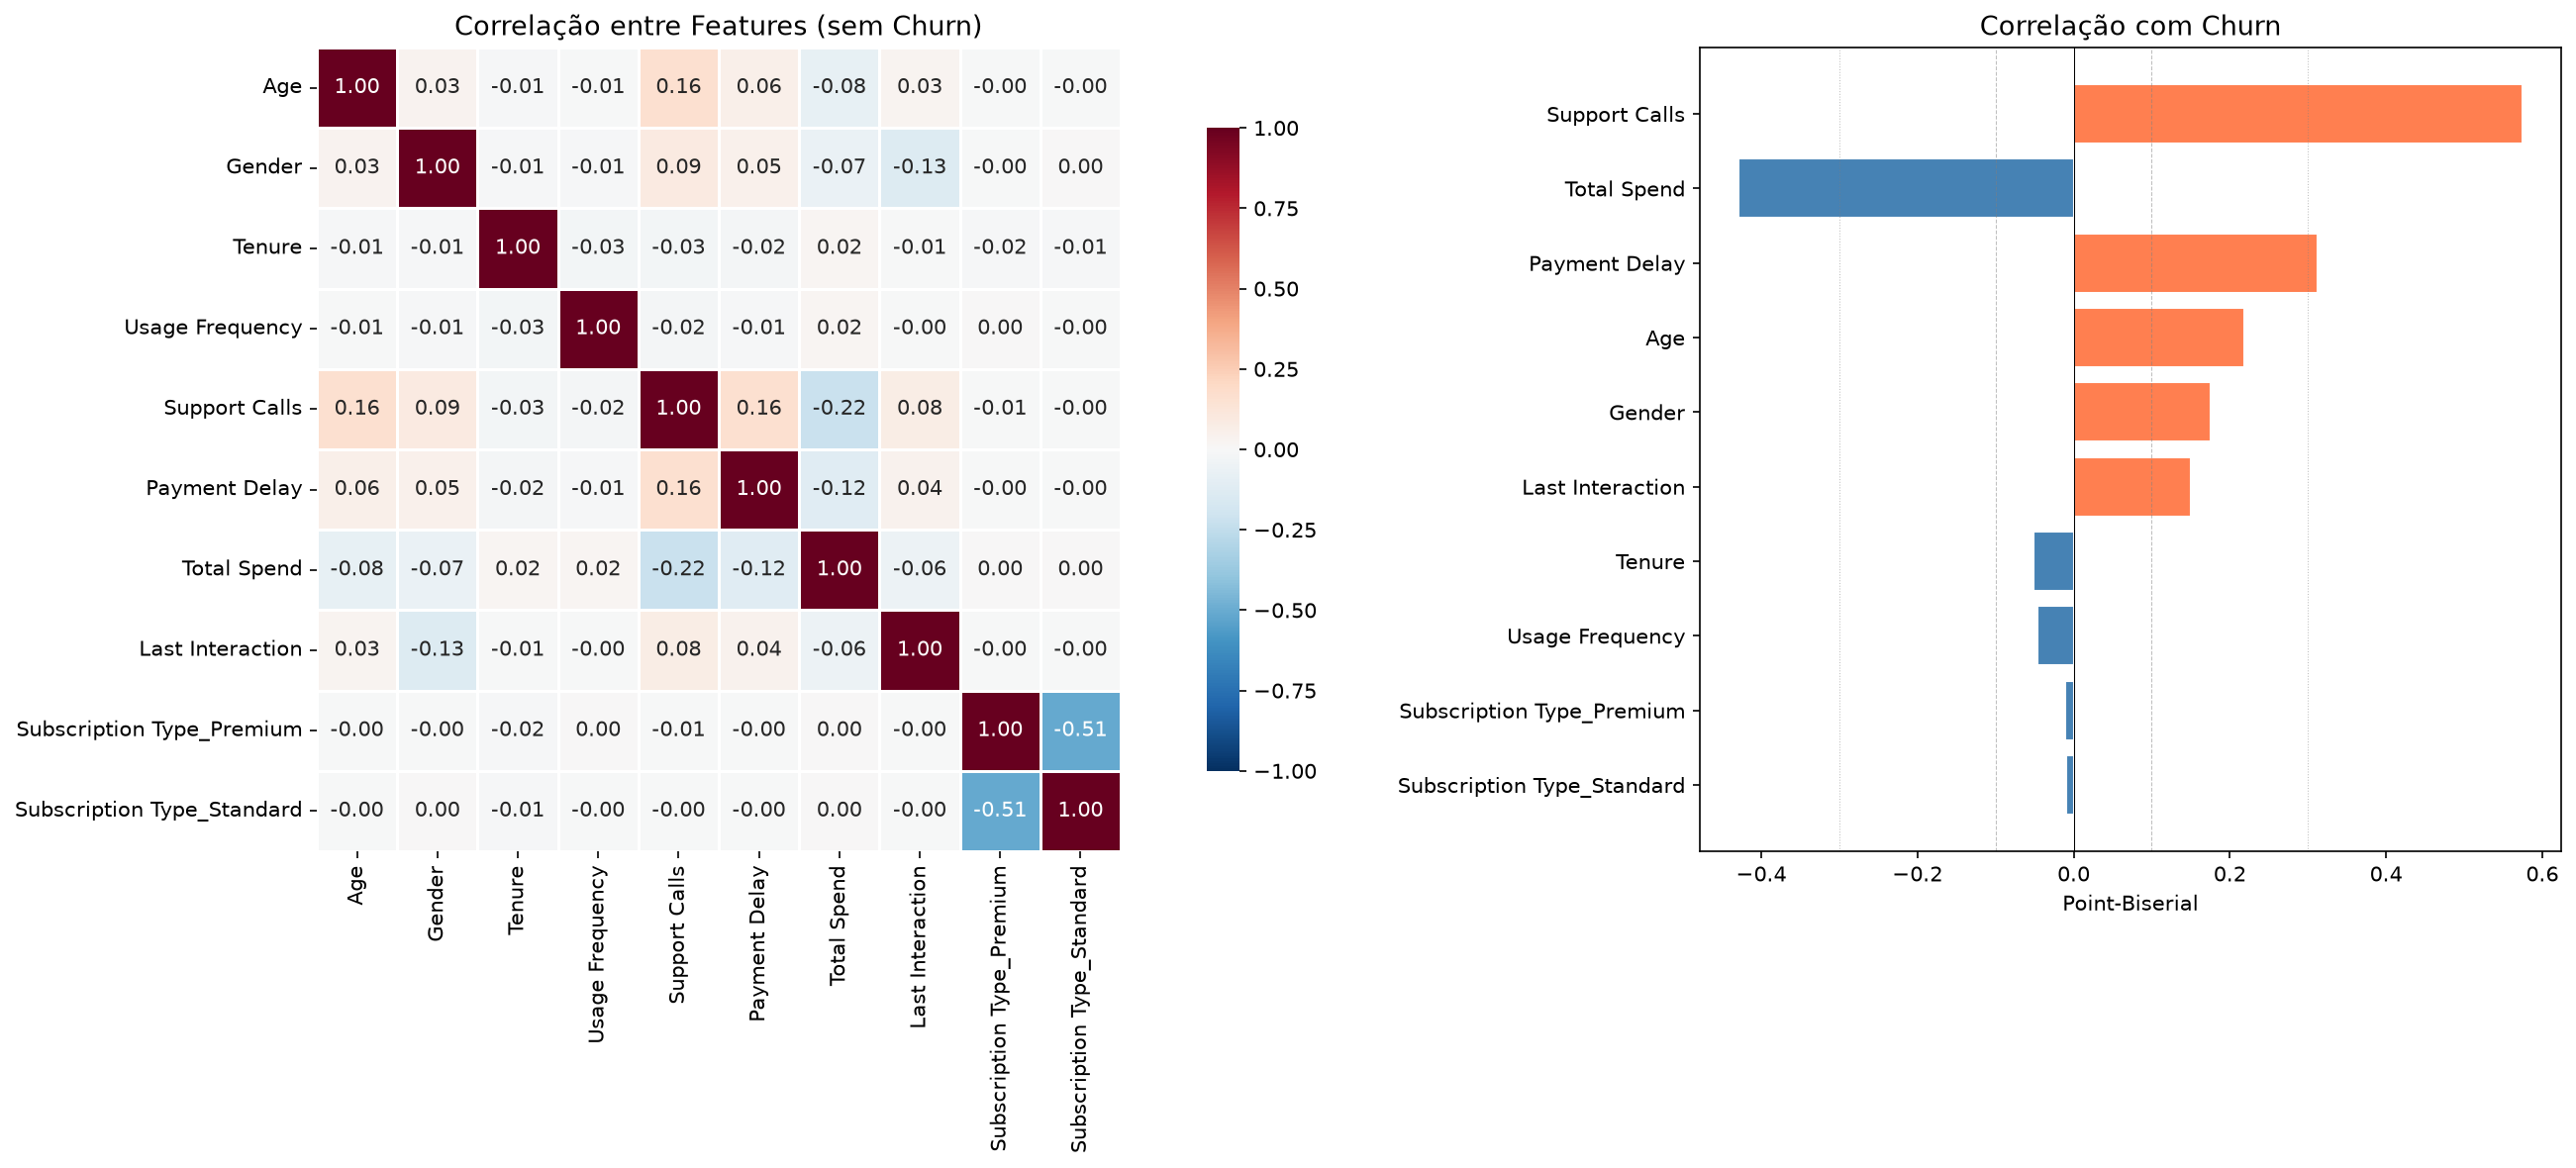
\includegraphics[width=\textwidth]{1_prep_correlacao_completa.png}
  \caption{À esquerda: matriz de correlação entre features. À direita: correlação
           Point-Biserial de cada feature com a variável alvo \texttt{Churn}.}
  \label{fig:corr}
\end{figure}

% -----------------------------------------------------------------------------
\subsection{Normalização e Exportação}

Após todas as transformações, o conjunto final conta com \textbf{10 features}.
Um \texttt{StandardScaler} foi ajustado exclusivamente no conjunto de treino e
aplicado ao teste (sem vazamento de informação). Os dados escalados foram exportados
no formato \textit{Parquet} e reutilizados por todos os notebooks de modelagem.

% =============================================================================
\section{Criação dos Modelos de Classificação}

\subsection{Metodologia Comum}

Todos os modelos seguiram o mesmo protocolo de treinamento e avaliação:

\begin{enumerate}
  \item O conjunto de treino (440.832 amostras) foi dividido em X\_tr (80\%) e
        X\_val (20\%), com estratificação pela variável alvo.

  \item Cada modelo foi treinado em X\_tr.

  \item O \textbf{threshold de decisão} foi calibrado no X\_val por meio da curva
        Precision-Recall: encontra-se o limiar que maximiza o F1 no conjunto de
        validação. Isso evita usar o threshold fixo 0,5, que se mostrou inadequado
        dado o desbalanceamento residual entre treino e teste.

  \item A avaliação final foi realizada no conjunto de teste (64.374 amostras),
        nunca utilizado durante o desenvolvimento.
\end{enumerate}

% -----------------------------------------------------------------------------
\subsection{SVM (Support Vector Machine)}

O SVM é um classificador baseado em margens: encontra o hiperplano que separa as
classes com a maior margem possível no espaço de features.

\subsubsection{Configuração}

Como o \texttt{LinearSVC} do scikit-learn não fornece probabilidades de saída,
ele foi encapsulado em um \texttt{CalibratedClassifierCV} com validação cruzada de
3 folds, o que adiciona a capacidade de estimar \texttt{predict\_proba} e viabiliza
a calibração do threshold.

\begin{table}[H]
  \centering
  \caption{Hiperparâmetros do SVM.}
  \begin{tabular}{ll}
    \toprule
    Parâmetro & Valor \\
    \midrule
    Tipo            & LinearSVC + CalibratedClassifierCV \\
    C (regularização) & 0,1 (regularização forte) \\
    class\_weight   & balanced \\
    max\_iter       & 2000 \\
    cv (calibração) & 3 folds \\
    \bottomrule
  \end{tabular}
  \label{tab:svm_params}
\end{table}

\subsubsection{Justificativa dos hiperparâmetros}

O valor $C = 0{,}1$ impõe regularização forte, penalizando menos o erro de
classificação em favor de uma margem mais ampla, o que tende a melhorar a
generalização diante de datasets com shift de distribuição. O \texttt{class\_weight='balanced'}
ajusta os pesos das classes automaticamente para compensar o desbalanceamento entre
as taxas de churn no treino (56,7\%) e no teste (47,4\%).

% -----------------------------------------------------------------------------
\subsection{MLP (MultiLayer Perceptron)}

A rede neural \textit{Multilayer Perceptron} é um classificador que aprende
representações hierárquicas das features por meio de camadas de neurônios com
funções de ativação não lineares.

\subsubsection{Arquitetura e Configuração}

\begin{table}[H]
  \centering
  \caption{Configuração da rede MLP.}
  \begin{tabular}{ll}
    \toprule
    Parâmetro & Valor \\
    \midrule
    Camadas ocultas      & 2 (64 → 32 neurônios) \\
    Função de ativação   & ReLU \\
    Solver               & Adam \\
    Learning rate inicial & 0,001 \\
    Regularização L2 ($\alpha$) & 0,01 \\
    Early stopping       & Sim (10\% do X\_tr como validação interna) \\
    Máx. de épocas       & 100 \\
    \bottomrule
  \end{tabular}
  \label{tab:mlp_params}
\end{table}

\subsubsection{Justificativa dos hiperparâmetros}

A arquitetura compacta (64 → 32) foi escolhida para equilibrar capacidade de
aprendizado e risco de overfitting dado o tamanho do dataset. A regularização
L2 com $\alpha = 0{,}01$ penaliza pesos grandes, reduzindo o overfitting. O
\textit{early stopping} interrompe o treinamento quando o desempenho no conjunto
de validação interna para de melhorar, evitando épocas desnecessárias.

A Figura~\ref{fig:mlp_loss} exibe a curva de perda ao longo das épocas de treinamento.

\begin{figure}[H]
  \centering
  
\includegraphics[width=0.75\textwidth]{2b_rn_loss_por_epoca.png}
  \caption{Curva de loss por época do MLP. O early stopping interrompe o treinamento
           quando o ganho adicional torna-se irrelevante.}
  \label{fig:mlp_loss}
\end{figure}

% -----------------------------------------------------------------------------
\subsection{AdaBoost}

O AdaBoost (\textit{Adaptive Boosting}) é um método de comitê que combina múltiplos
classificadores fracos de forma sequencial: cada estimador foca nos exemplos que o
anterior classificou incorretamente, aumentando seus pesos. O resultado final é uma
combinação ponderada de todos os estimadores.

\subsubsection{Configuração}

\begin{table}[H]
  \centering
  \caption{Hiperparâmetros do AdaBoost.}
  \begin{tabular}{ll}
    \toprule
    Parâmetro & Valor \\
    \midrule
    Número de estimadores & 200 \\
    Learning rate         & 0,05 \\
    Estimador base        & DecisionTreeClassifier (stump, max\_depth=1) \\
    \bottomrule
  \end{tabular}
  \label{tab:ada_params}
\end{table}

\subsubsection{Justificativa dos hiperparâmetros}

O \texttt{learning\_rate = 0{,}05} é conservador: cada estimador contribui menos
para a combinação final, forçando um aprendizado mais gradual e estável. Combinado
com 200 estimadores, esse ajuste favorece a convergência suave em detrimento de
uma convergência rápida que poderia levar a overfitting.

% =============================================================================
\section{Análise Comparativa do Desempenho dos Modelos}

\subsection{Métricas utilizadas}

Foram calculadas seis métricas para cada modelo no conjunto de teste:

\begin{itemize}
  \item \textbf{Balanced Accuracy:} $\frac{\text{Recall}_0 + \text{Recall}_1}{2}$.
        Métrica de ranking principal neste trabalho (ver justificativa abaixo).
  \item \textbf{Acurácia:} proporção de predições corretas.
  \item \textbf{Precision:} proporção de positivos preditos que são verdadeiros positivos.
  \item \textbf{Recall:} proporção de positivos reais corretamente identificados.
  \item \textbf{F1-Score:} média harmônica de Precision e Recall.
  \item \textbf{Kappa de Cohen:} concordância entre predições e gabarito descontando
        o acaso.
\end{itemize}

Dois classificadores triviais (\textit{Dummy}) foram incluídos como linha de base:
\textit{most\_frequent} (prevê sempre a classe majoritária) e \textit{stratified}
(prevê aleatoriamente respeitando a distribuição do treino). Um modelo real só é
útil se superar esses baselines.

\subsection{Por que Balanced Accuracy ao invés de F1-Score}

Com recall próximo de 1,0 e precision próxima de 0,5, o F1-Score fica artificialmente
inflado mesmo para modelos sem poder discriminativo real. O Dummy que prevê sempre
churn=1 obtém F1 = 0,643, valor quase idêntico ao MLP (F1 = 0,663) --- o F1 não
distingue o modelo do acaso nesse cenário. A Balanced Accuracy não é afetada por
esse viés: o mesmo Dummy obtém 0,500 (aleatoriedade pura), enquanto um modelo real
deve superar esse valor.

\subsection{Resultados}

A Tabela~\ref{tab:resultados} apresenta o desempenho de todos os classificadores
avaliados, ordenados por Balanced Accuracy. A Figura~\ref{fig:barplot} exibe o
comparativo visual.

\begin{table}[H]
  \centering
  \caption{Desempenho dos modelos no conjunto de teste (64.374 amostras),
           ordenados por Balanced Accuracy.}
  \label{tab:resultados}
  \setlength{\tabcolsep}{6pt}
  \begin{tabular}{lcccccc}
    \toprule
    \textbf{Modelo} & \textbf{Bal. Acc.} & \textbf{Acurácia} & \textbf{Precision}
                    & \textbf{Recall} & \textbf{F1} & \textbf{Kappa} \\
    \midrule
    \textbf{SVM}       & \textbf{0,604} & 0,584 & 0,533 & 0,984 & 0,691 & \textbf{0,200} \\
    AdaBoost           & 0,576 & 0,554 & 0,515 & 0,997 & 0,679 & 0,146 \\
    Árvore de Decisão  & 0,576 & 0,554 & 0,515 & 0,996 & 0,679 & 0,145 \\
    KNN                & 0,568 & 0,545 & 0,510 & 0,992 & 0,674 & 0,129 \\
    Random Forest      & 0,543 & 0,519 & 0,496 & 0,998 & 0,663 & 0,082 \\
    XGBoost            & 0,543 & 0,519 & 0,496 & 0,998 & 0,663 & 0,081 \\
    \textbf{MLP}       & 0,542 & 0,518 & 0,496 & 0,999 & 0,663 & 0,080 \\
    \midrule
    Dummy (most\_freq) & 0,500 & 0,474 & 0,474 & 1,000 & 0,643 & 0,000 \\
    Dummy (stratified) & 0,499 & 0,495 & 0,472 & 0,566 & 0,515 & $-$0,003 \\
    \bottomrule
  \end{tabular}
\end{table}

\begin{figure}[H]
  \centering
  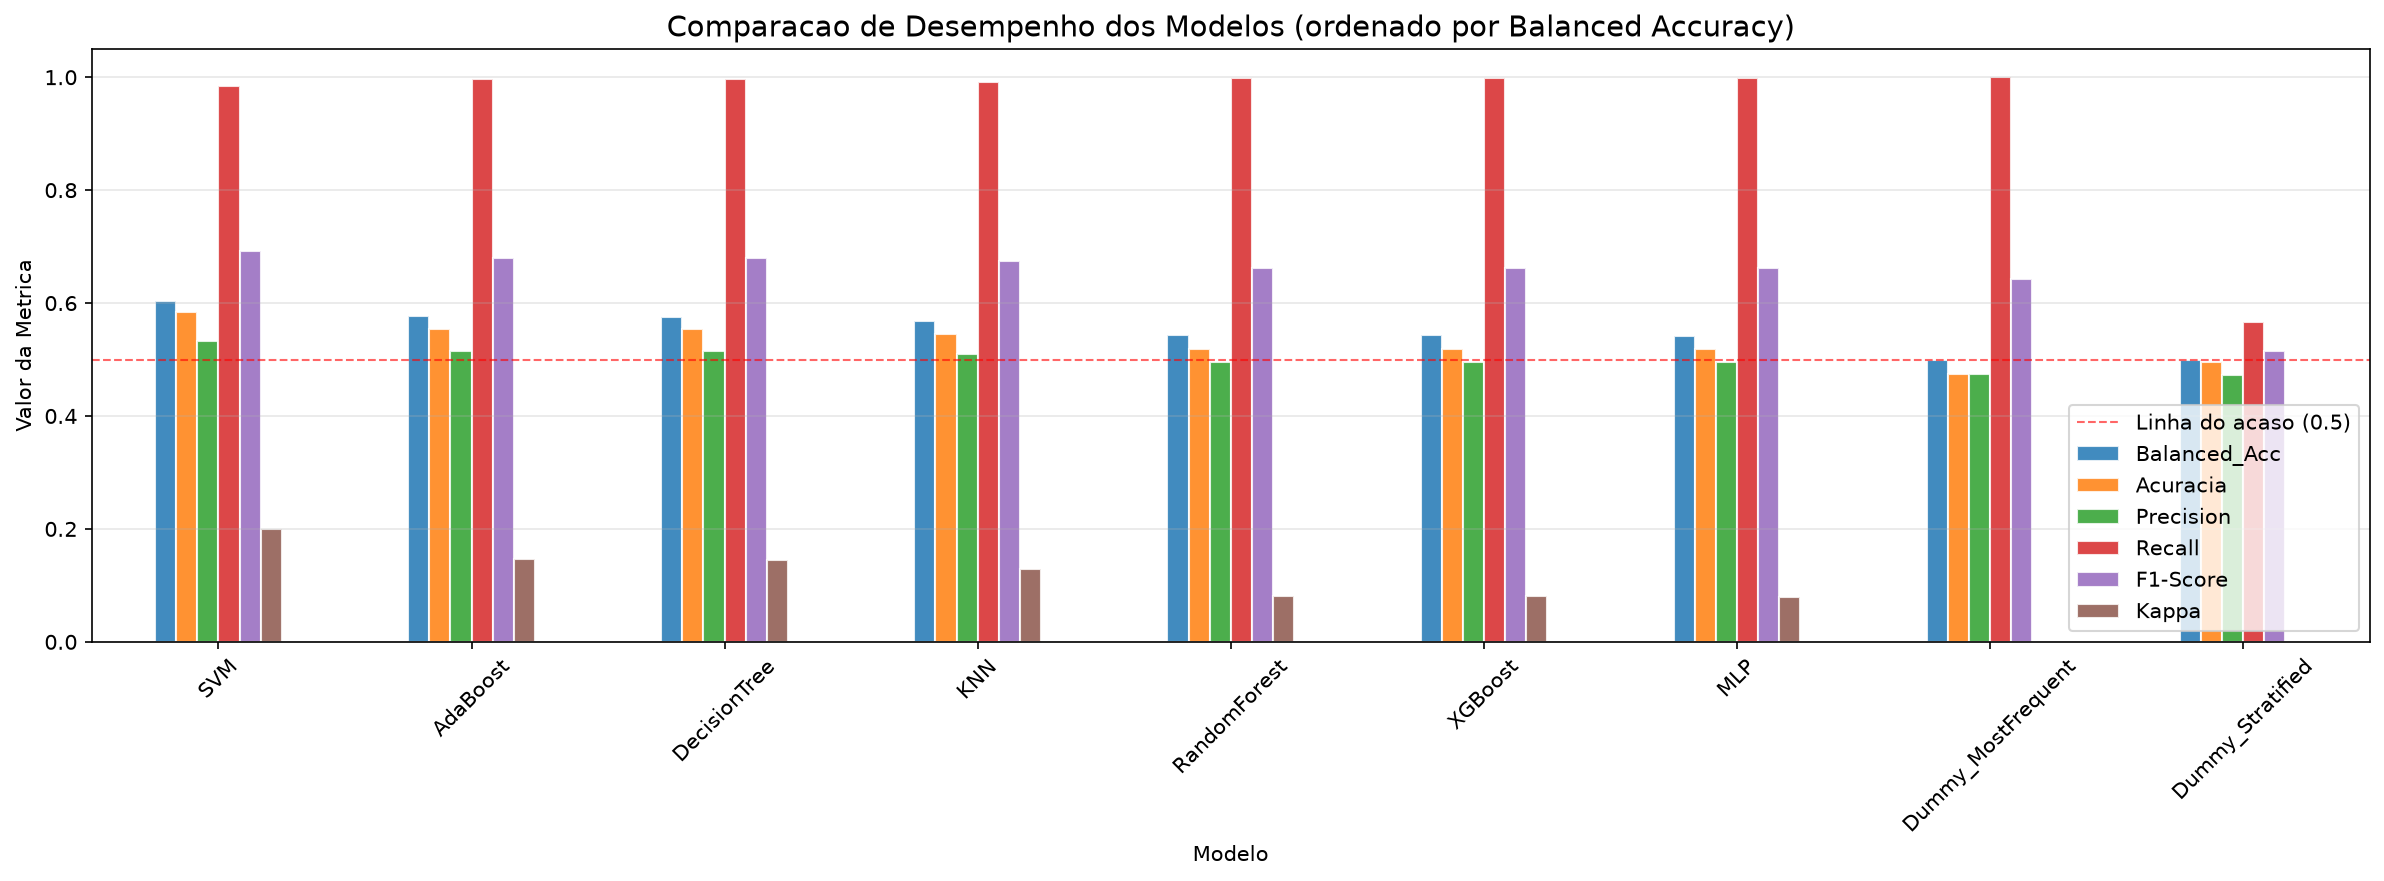
\includegraphics[width=\textwidth]{3_comp_barplot_metricas.png}
  \caption{Comparação das métricas de todos os modelos, ordenados por Balanced Accuracy.
           A linha vermelha tracejada marca o nível do acaso (0,500).}
  \label{fig:barplot}
\end{figure}

\subsection{Discussão}

\textbf{Todos os modelos reais superam os baselines.} A Balanced Accuracy de todos
os sete classificadores treinados está acima de 0,500 (limiar dos Dummies), confirmando
que os modelos aprenderam algum padrão genuíno nos dados.

\textbf{O SVM apresentou o melhor desempenho geral}, com Balanced Accuracy = 0,604
e Kappa = 0,200. Esse resultado está alinhado com o perfil dos dados: as correlações
Point-Biserial mostraram que a relação entre as features e o churn é predominantemente
linear, contexto em que classificadores baseados em hiperplano tendem a se sair bem.

\textbf{AdaBoost ocupou a segunda posição} (Balanced Acc = 0,576, Kappa = 0,146),
igualando a Árvore de Decisão simples. A sequência de estimadores fracos não trouxe
ganho expressivo sobre o modelo base neste dataset.

\textbf{MLP foi o pior dos três modelos escolhidos} (Balanced Acc = 0,542, Kappa = 0,080).
A rede neural exige mais dados ou features com padrões não-lineares relevantes para
superar modelos lineares; neste problema, o sinal disponível parece insuficiente para
explorar a capacidade extra da MLP.

\textbf{O recall elevado ($> 0{,}98$) em todos os modelos} indica que os thresholds
calibrados ainda são baixos (em torno de 0,35--0,45). Isso decorre de um distribution
shift residual: mesmo após a remoção do \texttt{Contract Length}, as distribuições
de \texttt{Support Calls} e \texttt{Payment Delay} ainda diferem entre treino e
teste (notado na EDA), fazendo com que as probabilidades estimadas pelos modelos
no conjunto de teste sejam sistematicamente mais altas do que o real.

% =============================================================================
\section{Conclusões, Comentários e Sugestões sobre o Trabalho}

\subsection{Conclusões}

O SVM com regularização forte ($C = 0{,}1$) e threshold calibrado mostrou-se o
modelo mais robusto para o problema de predição de churn neste dataset, atingindo
Balanced Accuracy = 0,604 e Kappa = 0,200 no conjunto de teste.

O principal desafio do trabalho não foi técnico, mas estrutural: o dataset apresenta
um \textit{distribution shift} severo na variável \texttt{Contract Length}, onde
contratos \textit{Monthly} têm 100\% de churn no treino mas comportamento radicalmente
diferente no teste. Identificar e tratar esse problema foi mais impactante do que
qualquer escolha de hiperparâmetro.

Os modelos mais simples (SVM linear, Árvore de Decisão) superaram os mais complexos
(MLP, Random Forest, XGBoost), o que é consistente com o perfil do problema: as
relações entre features e churn são predominantemente lineares, e os dados de teste
têm uma distribuição ligeiramente diferente do treino, favorecendo modelos com menor
capacidade de memorização.

\subsection{Comentários}

A métrica F1-Score, utilizada inicialmente como critério de ranking, se mostrou
inadequada neste contexto: com recall $\approx 1{,}0$ e precision $\approx 0{,}5$,
o F1 de um Dummy que prevê sempre a classe positiva atingiu 0,643 --- valor próximo
ao dos modelos reais. A substituição pelo Balanced Accuracy como métrica principal
revelou com mais clareza o nível real de discriminação de cada classificador.

A calibração de threshold via curva Precision-Recall no conjunto de validação foi
uma melhoria metodológica relevante: eliminou a dependência do limiar fixo de 0,5
e permitiu que cada modelo encontrasse seu ponto de equilíbrio próprio entre
Precision e Recall.

\subsection{Sugestões de Melhoria}

\begin{itemize}
  \item \textbf{Adversarial Validation:} treinar um classificador binário ``é amostra
        de treino ou de teste?''. Se o AUC for alto, há shift detectável que merece
        investigação antes da modelagem.

  \item \textbf{Busca de hiperparâmetros:} substituir valores fixos por
        \texttt{RandomizedSearchCV} com validação cruzada interna, garantindo que
        as escolhas sejam orientadas por evidência e não por julgamento manual.

  \item \textbf{Feature engineering:} criar features de interação como
        \texttt{Support Calls × Payment Delay} pode capturar padrões que as features
        isoladas não expressam.

  \item \textbf{Investigação da origem do shift:} a discrepância em
        \texttt{Contract Length} pode indicar um problema na coleta dos dados
        (viés de amostragem ou mudança temporal no perfil dos clientes) que
        deveria ser corrigido na fonte antes da modelagem.

  \item \textbf{Calibração de probabilidades (Platt Scaling):} além do threshold,
        calibrar as probabilidades brutas dos modelos melhoraria a qualidade das
        predições probabilísticas e permitiria comparações mais justas entre classificadores.
\end{itemize}

\end{document}
